\documentclass[../main.tex]{subfiles}
\begin{document}
\begin {definition} \label{modulo}
Sea $A$ un anillo, se llama $A$-módulo a cualquier grupo abeliano $(M,+)$ sobre el que $A$ actúa linealmente, es decir, un grupo $M$ con junto con una operación externa $A\times M \to M$ que cumple que para todo $m,n \in M, a,b \in A$:
\begin{enumerate}
  \item $a(m+n) = am + an$
  \item $(a+b)m = am+bm$
  \item $(ab)m = a(bm)$
  \item $1_Am = m$.
\end{enumerate}
\end{definition}

\begin{example}
\begin{enumerate}
  \item Si $\mathbb K $ es un cuerpo, todo $\mathbb K$-espacio vectorial es un $\mathbb K$-módulo..
  \item Si $V$ es un $\mathbb K$-espacio vectorial de dimensión finita y $f:V\to V$ un endomorfismo, entonces $V$ es un $\mathbb K[x]$-módulo via la aplicación

  \begin{align*}
    {\mathbb K[x]\times V} & \to     V                                 \\
    {(p(x),v)}             & \mapsto p(f) = a_nf^{(n)}+\dots+a_1 f+a_0
  \end{align*}
  siendo $p(x) = a_nx^n+\dots+a_1x + a_0$ y $f^(k) = f\circ \overset{k)}{\dots} \circ f$.
  \item Toda $A$-álgebra $B$ de un anillo $A$ es un $A$-módulo. $B$ es un anillo luego $(B,+)$ es un grupo abeliano. Por ser $A$-álgebra, existe un homomorfismo $\varphi:A\to B$, y entonces podemos definir la operación externa de la definición \ref{modulo} como $A\times B \to B$ que hace corresponder $(a,b) \mapsto\varphi(a)b$.
\end{enumerate}
\end{example}

\begin{remark} \label{prop_adicional}
Atendiendo al último ejemplo resulta que dados dos anillos $A, B$, dar a $B$ estructura de $A$-álgebra es equivalente a darle estructura de $A$-módulo junto con la propiedad adicional de que
\[\forall b, b' \in B, \; \forall a \in  A \quad a \cdot_{\text{ext}} (bb') = (a\cdot_{\text{ext}} b) b'\]
\end{remark}
\begin{definition}. Dado un anillo $A$ y un $A$-módulo $M$, diremos que $S\subset M$ es un \textit{submódulo de $M$} si es un subgrupo de $M$ cerrado para la multiplicación por elementos de $A$.
\end{definition}

\begin{remark} Si $A$ es un anillo, $\af\subseteq A$ un ideal, y $M$ un $A$-módulo entonces el conjunto$$\af M:=\left\{\sum_{i=1}^ra_im_i\ |\ r\in\N,\ a_i\in\af,\ m_i\in\N\right\}$$es un submódulo de $A$.
\end{remark}

\begin{definition}. Sean $(A,+,\cdot)$ anillo, $M$ y $N$ $A$-módulos. Una aplicación $f:M\longrightarrow N$ se dice que es un homomorfismo de $A$-módulos o, simplemente, que es una aplicación $A$-lineal si verifica
\begin{itemize}
    \item[\textit{i})] $\forall\ m_1,m_2\in M\hspace{15pt} f(m_1+m_2)=f(m_1)+f(m_2)$ y
    \item[\textit{ii})] $\forall\ \lambda\in A,\ \forall\ m\in M\hspace{15pt} f(\lambda m)=\lambda f(m).$
\end{itemize}
\end{definition}

\textbf{Observaciones}. \textit{\textit{i})} En un $A$-módulo $M$ se tiene que\begin{align*}
    &\forall\ m\in M \hspace{15pt}0_Am=0_M\\
    &\forall\ \lambda\in A \hspace{15pt}\lambda0_M=0_M.
\end{align*}
Para ver lo primero basta observar que para todo $m\in M$ se tiene que $0_Am+m=(0_A+1_A)m=1_Am=m$, es decir, $0_Am=0_M$. De aquí se desprende también que $$(-1_A)(1_M)=-1_M=(1_A)(-1_M)$$ puesto que $0_M=0_A1_M=(1_A-1_A)1_M=1_A1_M+(-1_A)(1_M)=1_M+(-1_A)(1_M)$.

También se desprende que, para $\lambda\in A$ y $m\in M$ fijados (arbitrarios), $\lambda0_M=\lambda(0_Am)=(\lambda0_A)m=0_Am=0_M$; esto es, la segunda propiedad.

\textit{ii}) Dado un homomorfismo de $A$-módulos, $f:M\longrightarrow N$, se tiene que $\ker(f):=\{x\in M\ |\ f(x)=0_N\}$ es un submódulo de $M$ y que $\text{im}(f):=\{y\in N\ |\ \exists\ x\in M\ \text{tal que}\ f(x)=y\}$ es un submódulo de $N$.

\section{Construcciones con $A$-módulos}
\subsection{Módulos cociente}
Dados $(A,+,\cdot)$ un anillo, $M$ un $A$-módulo y $N\subset M$ un submódulo. Denotemos para cada $m\in M$ como $[m]_N$ a la clase de $m$ en $M/N$. Tras esta consideración, se tiene que $M/N$ junto a la aplicación
$$\begin{array}{rcl}
    M/N\times M/N&\longrightarrow&M/N\\
    ([m_1]_N,[m_2]_N)&\longmapsto&[m_1+m_2]_N.
\end{array}$$
tiene estructura de grupo abeliano. Esto es así puesto que $(M,+)$ es un grupo abeliano y, por lo tanto, todo subgrupo suyo también lo es; es decir, todo subgrupo suyo será normal y el cociente será de nuevo abeliano.

\begin{definition}. Sean $(A,+,\cdot)$ un anillo, $M$ un $A$-módulo y $N\subseteq M$ un submódulo. Definiendo la aplicación
$$\begin{array}{rcl}
    A\times M/N&\longrightarrow&M/N\\
    (\lambda,[m])&\longmapsto&\lambda[m]_N:=[\lambda m]_N
\end{array}$$
dotamos a $M/N$ de estructura de $A$-módulo y lo denominamos \textit{módulo cociente}.
\end{definition}

\begin{remark} La aplicación natural
$$\begin{array}{rcl}
    M&\longrightarrow&M/N\\
    m&\longmapsto&[m]_N
\end{array}$$
es un homomorfismo de $A$-módulos.
\end{remark}
\begin{subsection}{Anuladores}
\begin{definition} Dados $A$ un anillo y $M$ un $A$-módulo, definimos el anulador de $A$ en $M$ como$$Anul_A M = \{\lambda\in A\ |\  \lambda\cdot m=0, \forall m\in M\}$$
\end{definition}

\begin{remark} \textit{i)} $Anul_A M$ es un ideal de $A$:

\begin{itemize}

     \item[1)]Dados $\lambda_1, \lambda_2\in Anul_A M$, para cada $m\in M$, $\lambda_1\cdot m=\lambda_2\cdot m=0$. Restando, se obtiene $(\lambda_1-\lambda_2)\cdot m=0 \rightarrow \lambda_1 -\lambda_2\in Anul_A M$
     \item[2)]Dado $\lambda\in Anul_AM$, para cada $\alpha\in A$ y para cada $m\in M$ se tiene $(\alpha\cdot\lambda)\cdot m=\alpha\cdot(\lambda\cdot m) =\alpha\cdot 0=0$, luego $\alpha\cdot\lambda\in Anul_AM$
\end{itemize}
Por tanto, $A/Anul_AM$ tiene estructura de anillo. Además, podemos ver a $M$ como un $A/Anul_AM$-módulo mediante la aplicación
$$\begin{array}{rcl}
    \faktor{A}{Anul_AM}\times M&\longrightarrow&M\\
    (\lambda + Anul_AM)\cdot m&\longmapsto&\lambda\cdot m
\end{array}$$
\textit{ii)} Dado un ideal $\mathfrak{a}\subset Anul_AM$, $M$ es un $A/\mathfrak{a}$-módulo. Los submódulos de $M$ como $A/\mathfrak{a}$-módulo son los submódulos de $M$ como $A$-módulo.
\end{remark}
\end{subsection}
\begin{subsection}{Aplicaciones A-lineales}
\begin{definition}. Dados $M$ y $N$ dos $A$-módulos, definimos \textit{el conjunto de aplicaciones $A$-lineales entre $M$ y $N$}
$$\Hom_A(M,N):=\{f:M\longrightarrow N\ |\ f\text{ es aplicación }A\text{-lineal}\}
$$
\end{definition}
\textbf{Proposición}. Dados $M$ y $N$ dos $A$-módulos, $\Hom_A(M,N)$ tiene estructura de $A$-módulo.

Demostración. En primer lugar, definamos para cada $\lambda\in A$ y cada $f\in\Hom_A(M,N)$ la aplicación
$$\begin{array}{rccl}
    \lambda f:&M&\longrightarrow&N\\
    &m&\longmapsto&\lambda(f(m))
\end{array}$$
y veamos de nuevo que $\lambda f\in\Hom_A(M,N)$, de forma que
$$\begin{array}{rcl}
    A\times\Hom_A(M,N)&\longrightarrow&\Hom_A(M,N)\\
    (\lambda,f)&\longmapsto&\lambda f
\end{array}$$
esté bien definida. Sean $m,m_1,m_2\in M$ y $\mu\in A$:
\begin{align*}
    (\lambda f)(m_1+m_2)&=\lambda(f(m_1+m_2))=\\
    &=\lambda(f(m_1)+f(m_2))=\\
    &=\lambda(f(m_1))+\lambda(f(m_2))=(\lambda f)(m_1)+(\lambda f)(m_2).
\end{align*}
\begin{align*}
    (\lambda f)(\mu m)&=\lambda(f(\mu m))=\lambda(\mu(f(m)))=(\lambda\mu)(f(m))=\\
    &=(\mu\lambda)(f(m))=\mu(\lambda(f(m)))=(\mu(\lambda f))(m).
\end{align*}
Ahora, dadas $f,g\in\Hom_A(M,N)$ definamos la aplicación
$$\begin{array}{rccl}
    f+g:&M&\longrightarrow&N\\
    &m&\longmapsto&f(m)+g(m)
\end{array}$$
Veamos que $f+g\in\Hom_A(M,N)$. Dados $m,m_1,m_2\in M$ y $\lambda\in A$ arbitrarios, tenemos efectivamente
\begin{align*}
    (f+g)(m_1+m_2)&=f(m_1+m_2)+g(m_1+m_2)=\\
    &=f(m_1)+f(m_2)+g(m_1)+g(m_2)=(f+g)(m_1)+(f+g)(m_2).
\end{align*}
\begin{align*}
    (f+g)(\lambda m)&=f(\lambda m)+g(\lambda m)=\lambda f(m)+\lambda g(m)=\\
    &=\lambda(f(m)+g(m))=\lambda((f+g)(m))=(\lambda(f+g))(m).
\end{align*}
Así,
$$\begin{array}{rrcl}
    +:&\Hom_A(M,N)\times\Hom_A(M,N)&\longrightarrow&\Hom_A(M,N)\\
    &(f,g)&\longmapsto&f+g,
\end{array}$$
está bien definida y dota a $\Hom_A(M,N)$ de estructura de grupo abeliano.

Comprobemos por último que el producto exterior cumple los cuatro axiomas de la definición de $A$-módulo. Sean $m\in M$, $f,g\in\Hom_A(M,N)$ y $\lambda,\mu\in A$ arbitrarios:
\begin{itemize}
    \item[\textit{i})] $(\lambda(f+g))(m)=\lambda((f+g)(m))=\lambda(f(m)+g(m))=\lambda(f(m))+\lambda(g(m))=(\lambda f)(m)+(\lambda g)(m)=(\lambda f+\lambda g)(m)$,
    \item[\textit{ii})] $((\lambda+\mu)f)(m)=(\lambda+\mu)(f(m))=\lambda(f(m))+\mu(f(m))=(\lambda f)(m)+(\mu f)(m)=(\lambda f+\mu f)(m)$,
    \item[\textit{iii})] $((\lambda\mu)f)(m)=(\lambda\mu)(f(m))=\lambda(\mu(f(m))=\lambda((\mu f)(m))=(\lambda(\mu f))(m)$ y
    \item[\textit{iv})] $(1_A f)(m)=1_A(f(m))=f(m)$.
\end{itemize}
\end{subsection}
\begin{subsection}{Pullbacks}
Dados $M_1$, $M_2$ y $N$ $A$-módulos y dada $\varphi\in\Hom_A(M_1,M_2)$, podemos definir
$$\begin{array}{rrcl}
    \varphi^{\ast}:&Hom_A(M_2,N)&\longrightarrow&Hom_A(M_1,N)\\
    &g&\longmapsto&g\circ\varphi
\end{array}$$ que resulta ser un homomorfismo de $A$-módulos y se denota $\varphi^{\ast}=Hom_A(\varphi\_)$.

Análogamente, dados $M$, $N_1$ y $N_2$ $A$-módulos y dada $\psi\in\Hom_A(N_1,N_2)$,
$$\begin{array}{rrcl}
    \psi^{\ast}:&Hom_A(M,N_1)&\longrightarrow&Hom_A(M,N_2)\\
    &g&\longmapsto&\psi\circ g
\end{array}$$
es un homomorfismo de $A$-módulos.

Nótese que si tenemos $M_1$, $M_2$ y $M_3$ $A$-módulos y $\varphi\in Hom_A(M_1,M_2)$ y $\psi\in Hom_A(M_2,M_3)$, entonces $(\psi\circ\varphi)^{\ast}=\varphi^{\ast}\circ\psi^{\ast}$
\end{subsection}
\begin{subsection}{Suma directa}
\begin{definition}. Sean $(A,+,\cdot)$ un anillo conmutativo unitario y $\{M_i\}_{i\in I}$ una familia no vacía de $A$-módulos. Definimos el conjunto
$$
\bigoplus_{i\in I}M_i:=\left\{{(m_i)}_{i\in I}\in\prod_{i\in I}M_i\ |\ m_i=0_{M_i},\forall\ i\in I\setminus F,\ F\subseteq I\ \text{finito}\right\}
$$
y lo llamamos \textit{suma directa} de los $A$-módulos $\{M_i\}_{i\in I}$.
\end{definition}

\textbf{Proposición}. Sean $A$ un anillo y una familia $\{M_i\}_{i\in I}$ de $A$-módulos. Definamos las aplicaciones
$$\begin{array}{rrcl}
    +:&\bigoplus_{i\in I}M_i\times\bigoplus_{i\in I}M_i&\longrightarrow&\bigoplus_{i\in I}M_i\\
    &({(m_i)}_i,{(m'_i)}_i)&\longmapsto&{(m_i)}_i+{(m'_i)}_i:={(m_i+m'_i)}_i,
\end{array}$$
y
$$\begin{array}{rcl}
    A\times\bigoplus_{i\in I}M_i&\longrightarrow&\bigoplus_{i\in I}M_i\\
    (\lambda,{(m_i)}_i)&\longmapsto&\lambda{(m_i)}_i:={(\lambda m_i)}_i.
\end{array}$$
Se tiene que $(\bigoplus_{i\in I}M_i,+)$ es un grupo abeliano y $\bigoplus_{i\in I}M_i$ es un $A$-módulo mediante el producto exterior definido.

\textbf{Observaciones}. \textit{\textit{i})} Para cada $j\in I$, tenemos definida $p_j:\bigoplus_{i\in I}M_i\rightarrow M_j$, la proyección a cada $M_j$. No es más que la restricción a $\bigoplus_{i\in I}M_i$ de la proyección $\Pi_j$ definida sobre el producto cartesiano $\Pi_{i\in I}M_i$. $p_j$ es un homomorfismo de $A$-módulos.

\textit{ii)} Para cada $j\in I$, definimos la inclusión
$$\begin{array}{rrcl}
q_j:&M_j&\longrightarrow&\bigoplus_{i\in I}M_i\\
&x&\longmapsto&  (x) := \left\{ \begin{array}{ll}
         0 & \mbox{si $i\neq j$};\\
         x & \mbox{si $i=j$}.\end{array} \right.
\end{array}$$

$q_j$ es un homomorfismo de anillos.

\textit{iii)} Para cada $x=(x_i)\in \bigoplus_{i\in I}M_i$, existe un número finito de índices $i_1,...,i_r$ tal que $x_{i_r}\neq 0$. Entonces, expresamos $x=\sum_{i\in {i_{i_1},...i_{i_r}}} q_i(x_i)$.

\textbf{Notación.} Dado $A$ un anillo, $I$ un conjunto no vacío, denotamos $A^{(I)}=\bigoplus_{i\in i} A_i$, donde para cada $i\in I$, $A_i=A$. $A^{(I)}$ es un submódulo de $A^{I} = \prod_{i\in I} A_i$, con $A_i=A$ para cada $i\in I$.
\end{subsection}
\section{A-módulos libres}

\begin{definition}. Dado un homomorfismo de $A$-módulos, $f:M\rightarrow N$, se dice que es un isomorfismo de $A$-módulos si existe $g:N\rightarrow M$ homomorfismo de $A$-módulos tal que $g\circ f = Id_M$ y $f\circ g = Id_N$, es decir, una inversa de $f$.
\end{definition}

\begin{remark} $f:M\longrightarrow N$ es isomorfismo de $A$-módulos si, y sólo si, es inyectivo y sobreyectivo. Esto significa que es suficiente que $f$ sea biyectivo como $A$-aplicación.
\end{remark}

\begin{lemma} Sean ${M_i:i\in I}$ un conjunto de $A$-módulos y sea $N$ otro $A$-módulo. Un homomorfismo $\Phi:\bigoplus_{i\in I} M_i \rightarrow N$ viene unívocamente determinado por los homomorfismos $\Phi \circ q_i:M_i \rightarrow N$. Análogamente, los homomorfismos $\Phi:N\rightarrow \bigoplus_{i\in I} M_i$ vienen unívocamente determinados por los homomorfismos $p_i\circ \Phi:N\rightarrow M_i$.
\end{lemma}

Demostración. Sea $\Phi:\bigoplus_{i\in I} M_i \rightarrow N$ un homomorfismo de $A$-módulos. Para cada $i\in I$, $\Phi \circ q_i$ es una composición de homomorfismos, luego es un homomorfismo de anillos.

Recíprocamente, dados $\Phi_i:M_i\rightarrow N$ homomorfismo de $A$-módulos, para cada $i\in I$, definimos $\Phi:\bigoplus_{i\in I} M_i\rightarrow N$ de la siguiente forma:

Para cada $\omega \in \bigoplus_{i\in I} M_i$, existen unos únicos $i_1,...,i_r$, todos ellos distintos, tales que $\omega=q_{i_1}(\omega_{i_1})+\cdots q_{i_r}(\omega_{i_r})$. Entonces, ponemos $\Phi(\omega)=\Phi_{i_1}(\omega_{i_1})+...+\Phi_{i_r}(\omega_{i_r})$. En el caso en el que $\omega$ sea $0$, ponemos $\Phi(\omega)=0$. $\Phi$ es un homomorfismo de anillos que cumple $\Phi\circ q_i = \Phi_i$, para cada $i\in I$.

\textbf{Notación}. Denotamos al $\Phi$ de la demostración anterior como $\bigoplus_{i\in I} \Phi_i$

\begin{proposition} Sea $A$ un anillo y $M$ un $A$-módulo. Son equivalentes
\begin{itemize}
    \item[1)] Existe $B:={\{m_i\}}_{i\in I}\subseteq M$ tal que para cada $x\in M$ existe $F\subseteq I$ cumpliendo que $x$ se puede expresar de forma única como$$x=\underset{\lambda_j\in A}{\sum_{j\in F}}\lambda_j m_j$$ y
    \item[2)] $M\approx A^{(I)}$.
\end{itemize}
Si se da cualquiera de ellas se dice que $M$ es un \textit{$A$-módulo libre} y $B$ es una base. Además, en estas condiciones, dos bases $B$ y $B'$ de $M$ tienen el mismo cardinal, que se llama \textit{rango de $M$}.
\end{proposition}

Demostración. $(1\Rightarrow 2)$ En primer lugar, para cada $i\in I$ definimos las aplicaciones
$$\begin{array}{rccl}
    \varphi_i:&A&\longrightarrow&M\\
    &1_A&\longmapsto&m_i.
\end{array}$$
por definición, para cada $i\in I$ y cada $\lambda\in A$ se verifica $\varphi_i(\lambda)=\lambda m_i$.
De esta forma, $\varphi_i$ es un homomorfismo de $A$-módulos entre $A$ y $M$ para cada $i\in I$ y, por el lema previo, $\varphi:=\bigoplus_{i\in I}\varphi_i: A^{(I)}\longrightarrow M$ es a su vez un homomorfismo de $A$-módulos.

Por otro lado, dado que por hipótesis todo $x\in M$ admite una representación única como combinación lineal finita de elementos de $B$, definimos para cada $i\in I$ las aplicaciones
$$\begin{array}{rccl}
    \psi_i:&M&\longrightarrow&A\\
    &x&\longmapsto&\lambda_i,
\end{array}$$
donde $\lambda_i$ es el correspondiente escalar asociado al elemento $m_i$ en la representación de $x$. De nuevo, para cada $i\in I$, $\psi_i$ es un homomorfismo de $A$-módulos y, de forma análoga, la aplicación
$$\begin{array}{rccl}
    \psi:&M&\longrightarrow&A^I
\end{array}$$
verificando $p_i\circ\psi=\psi_i$ es un homomorfismo de $A$-módulos y es único. Más aún, para cada $x\in M$ existe $F\subseteq I$ finito de forma que, $\psi_i(x)=0_A$ si $i\in I\setminus F$; es decir, $\psi(M)\subseteq A^{(I)}$.

Por último, es claro por definición de los homomorfismos que $\varphi\circ\psi=Id_{M}$ y $\psi\circ\varphi=Id_{A^{(I)}}$.

$(2\Rightarrow 1)$ Supongamos que existe $\phi: A^{(I)}\rightarrow M$ un isomorfismo de $A$-módulos, para cierto conjunto de índices $I$. Sea, para cada $i\in I$, $m_i:=\phi(e_i)$, donde $e_i\in A^{(I)}$ viene dado por
$$\begin{array}{rccl}
    e_i= \left\{ \begin{array}{ll}
         e_{ij}=0 & \mbox{si $i\neq j$};\\
         e_{ii}=1_A & \mbox{}\end{array} \right.
\end{array}$$
Veamos que ${m_i:i\in I}$ verifica 1). Para cada $m\in M$, por ser $\phi$ sobreyectiva, existe un $\underline{x}\in A^{(I)}$ tal que $\phi(\underline{x})=m$. A su vez, existen $i_1,...,i_r\in I$ tales que $\underline{x}=q_{i_1}(x_{i_1})+...+q_{i_r}(x_{i_r})=x_{i_1}q_{i_1}(1_A)+...+x_{i_r}q_{i_r}(1_A)$. Por tanto, $\phi(\underline{x})=x_{i_1}\phi(e_{i_1})+...+x_{i_r}\phi(e_{i_r})=x_{i_1}m_{i_1}+...+x_{i_1}m_{i_r}=m$. Hemos escrito $m$ como una combinación lineal de elementos ${m_i:i\in I}$

Supongamos ahora que para ciertos ${\{i_j\}}_{j\in\{1,\dots,r\}}\subset I$$$\lambda_{i_1}m_{i_1}+\cdots+\lambda_{i_r}m_{i_r}=0_M,\hspace{15pt}\lambda_{i_j}\in A.$$
Por ser así, tenemos
$$\Phi(\lambda_{i_1}e_{i_1}+\cdots+\lambda_{i_r}e_{i_r})=0_M\Longleftrightarrow\lambda_{i_1}e_{i_1}+\cdots+\lambda_{i_r}e_{i_r}=0_{A^{(I)}}\Longleftrightarrow\lambda_{i_j}=0_A\hspace{15pt}\forall\ j\in\{1,\dots,r\}.$$

Falta ver que todas las bases tienen un mismo cardinal. Para ello, usaremos las observaciones previas a la proposición.

Supongamos $M\approx A^{(I)}$. Sean $\mathfrak{m}$ un ideal maximal de $A$ (sabemos que existe) y ${\{m_i\}}_{i\in I}$ una base de $M$.
Tenemos que $\mathfrak{m}M$ es un submódulo de $M$ y, como $\mathfrak{m}\subset\Ann_A\left(\faktor{M}{\mathfrak{m}M}\right)$, $\faktor{M}{\mathfrak{m}M}$ tiene estructura de $\faktor{A}{\mathfrak{m}}$-espacio vectorial.

Tomemos $M=A^{(I)}$ y veamos que $\faktor{A^{(I)}}{\mathfrak{m}A^{(I)}}\approx\left(\faktor{A}{\mathfrak{m}}\right)^{(I)}$, que es un $\faktor{A}{\mathfrak{m}}$-espacio vectorial de dimensión $\#(I)$.

En primer lugar, definamos para cada $i\in I$ las siguientes aplicaciones
$$\begin{array}{rrcl}
\tau_i:&A&\longrightarrow&\left(\faktor{A}{\mathfrak{m}}\right)^{(I)}\\
&1_A&\longmapsto&\tau_i(1_A)={(a_j+\mathfrak{m})}_{j\in I}:=\left\{\begin{array}{lc}
a_j+\mathfrak{m}=\mathfrak{m}&\text{si }i\neq j\\
a_j+\mathfrak{m}=1+\mathfrak{m}&\text{si }i=j
\end{array}\right.
\end{array}.$$
Se comprueba que, para cada $i\in I$, $\tau_i$ es homomorfismo de $A$-módulos y, por lo tanto, $\bigoplus_{i\in I}\tau_i:A^{(I)}\longrightarrow\left(\faktor{A}{\mathfrak{m}}\right)^{(I)}$ es también un homomorfismo de $A$-módulos.

Además, $\bigoplus_{i\in I}\tau_i$ es sobreyectivo y $\ker{\bigoplus_{i\in I}\tau_i}=\mathfrak{m}A^{(I)}$. Así, por el Primer Teorema de Isomorfía, $\bigoplus_{i\in I}\tau_i$ induce un isomorfismo de $\faktor{A}{\mathfrak{m}}$-módulos, $\widehat{\bigoplus_{i\in I}\tau_i}:\faktor{A^{(I)}}{\mathfrak{m}A^{(I)}}\longrightarrow\left(\faktor{A}{\mathfrak{m}}\right)^{(I)}$

Ahora, dados dos conjuntos de índices no vacíos $I$ y $J$, supongamos que existe un isomorfismo de $A$-módulos $\Phi:A^{(I)}\longrightarrow A^{(J)}$. Por ser así, en concreto se tiene que $\Phi(\mathfrak{m}A^{(I)})=\mathfrak{m}A^{(J)}$ y $\Phi$ induce otro isomorfismo de $\faktor{A}{\mathfrak{m}}$-módulos, $\widehat{\Phi}:\faktor{A^{(I)}}{\mathfrak{m}A^{(I)}}\longrightarrow\faktor{A^{(J)}}{\mathfrak{m}A^{(J)}}$. De esta forma, resulta que $(\faktor{A}{\mathfrak{m}})^(I)\approx(\faktor{A}{\mathfrak{m}})^(J)$ y $\#(I)=\#(J)$.

\textbf{Corolario}. Sea $M$ es un $A$-módulo libre, es decir, existe un conjunto $I$ tal que $M\cong A^{(I)}$, y sea $N$ otro $A$-módulo. Dados ${n_i:i\in I}\subset N$, existe un único homomorfismo de $A$-módulos $f:M\rightarrow N$ tal que $f(m_i)=n_i$ para cada $i\in I$, donde ${m_i: i\in I}$ es una base de $M$

\section{Sucesiones exactas}

\begin{definition} Una sucesión de homomorfismos de $A$-módulos$$...\longrightarrow M_{i-1}\overset{\Phi_{i-1}}{\longrightarrow} M_i\overset{\Phi_i}{\longrightarrow}M_{i+1}\longrightarrow...$$ se dice exacta si $ker(\Phi_{i+1})=im(\Phi_i)$, donde para cada $i$, $M_i$ es un $A$-módulo y $\Phi_i:M_i\rightarrow M_{i+1}$ es un homomorfismo de $A$-módulos.
\end{definition}
\begin{definition} Decimos que una sucesión de homomorfismos de $A$-módulos es corta si es de la forma$$0\longrightarrow M_1\overset{f}{\longrightarrow} M_2\overset{g}{\longrightarrow} M_3\longrightarrow 0$$
\end{definition}
\begin{remark} Una sucesión corta es exacta si y sólo si $f:M_1\rightarrow M_2$ es inyectiva, $g:M_2\rightarrow M_3$ es suprayectiva y $im(f)=ker(g)$
\end{remark}
\begin{example} \textit{1)} Dados $N\subset M$ $A$-módulos,$$0\longrightarrow N\longrightarrow M\longrightarrow\faktor{M}{N}\longrightarrow 0$$ es una sucesión corta exacta.

	\textit{2)} Dados $M$ y $N$ $A$-módulos,$$0\longrightarrow M\overset{q_M}{\longrightarrow} M\oplus N\overset{p_N}{\longrightarrow} N\longrightarrow 0$$ es una también una sucesión corta exacta.
\end{example}
\begin{remark} Toda sucesión de homomorfismos de $A$-módulos se puede descomponer en varias sucesiones cortas.
\end{remark}
\begin{definition} Dado $M$ un $A$-módulo, un subconjunto $S\subset M$ es un sistema de generadores de $M$ si para cada $x\in M$ existen $\{s_1,...,s_n\}\subset S$ tales que$$x=\lambda_1s_1+...+\lambda_ns_n$$ con $\lambda_i\in A$ para cada $i\in\{1,...,n\}$.

	Es decir, el menor submódulo de $M$ que contiene a $S$ es el propio $M$.
\end{definition}
\begin{definition} Dado un conjunto de $A$-módulos $\zeta$, una aplicación $\lambda:\zeta\rightarrow\mathbb{N}$ se dice aditiva si para cada $M$, $M'$ y $M''\in\zeta$ y para cada sucesión corta y exacta$$0\longrightarrow M'\longrightarrow M\longrightarrow M''\longrightarrow 0$$ se verifica $\lambda(M) = \lambda(M')+\lambda(M'')$.
\end{definition}
\begin{example} Dado $K$ cuerpo, los $K$-módulos son los $K$-espacios vectoriales. Tomando $\zeta$ como los $K$-espacios vectoriales de dimensión finita,
	$$\begin{array}{rcl}
	\zeta&\longrightarrow&\mathbb{N}\\
	M&\longmapsto&dim(M)
	\end{array}$$
	es una aplicación aditiva.
\end{example}
\begin{proposition}\label{esc} Sea$$0\longrightarrow M'\overset{f}{\longrightarrow} M\overset{g}{\longrightarrow} M''\longrightarrow 0$$ una sucesión corta y exacta de $A$-módulos. Son equivalentes:
	\begin{itemize}
		\item [i)] Existe $\pi:M\longrightarrow M'$ homomorfismo de $A$-módulos tal que $\pi\circ f=1_{M'}$
		\item[ii)] Existe $\sigma:M''\longrightarrow M$ homomorfismo de $A$-módulos tal que $g\circ\sigma=1_{M''}$
		\item[iii)] $M\cong M'\oplus M''$ vía $f$ y $g$, es decir, existe $\Phi:M\longrightarrow M'\oplus M''$ isomorfismo de $A$-módulos tal que los diagramas son conmutativos.
	\end{itemize}
	En tal caso, se dice que la sucesión corta es escindida.
\end{proposition}

\begin{proof} $(1\Rightarrow 2)$ Dado $m''\in M''$, por ser $g$ sobreyectiva existe $m\in M$ tal que $g(m)=m''$. Considero $$m^*:=m-f\circ\tau(m)\in M$$
	y afirmo que $m^*$ no depende de la elección hecha de $m\in M$ de forma que $g(m)=m''$. Supongamos que existe otro $m_1\in M$ tal que $g(m_1)=m''$. Por ser así,
	$$g(m-m_1)=g(m)-g(m_1)=0_{M''}.$$
	Como $\ker (g)=\text{im} (f)$, existe $m'\in M'$ tal que $f(m')=m-m_1$. Dado que por hipótesis $\tau\circ f=\text{id}_{M'}$, tenemos
	$$m-m_1=f(m')=f\circ\tau(m-m_1)=f\circ\tau(m)-f\circ\tau(m_1)$$
	y
	$$m-f\circ\tau(m)=m_1-f\circ\tau(m_1).$$
	Vemos así que $m^*$ no depende del $m\in M$ escogido con tal de que se tenga $g(m)=m''$.

	Por esto que acabamos de ver, la aplicación
	$$\begin{array}{rrcl}
	\sigma:&M''&\longrightarrow&M\\
	&m''&\longmapsto&m^*=m-f\circ\tau(m)
	\end{array},$$
	donde $m$ verifica $g(m)=m''$, está bien definida. Además, para cada $m''\in M''$,
	$$g\circ\sigma(m'')=g(\sigma(m''))=g(m-f\circ\tau(m))=g(m)=m'',$$
	es decir, $g\circ\sigma=\text{id}_{M''}$.

	Falta por comprobar que $\sigma$ es homomorfismo de $A$-módulos. Sean $\lambda,\mu\in A$ y $m_1'',m_2''\in M''$ arbitrarios.
	Usamos que $f,g$ y $\tau$ son homomorfismos de $A$-módulos. en primer lugar, es claro que, si $m_1,m_2\in M$ verifican $g(m_i)=m_i''$, entonces $g(\lambda m_1)=\lambda m_1''$, $g(\mu m_2)=\mu m_2''$ y $g(\lambda m_1+\mu m_2)=\lambda m_1''+\mu m_2''$. Teniendo esto en cuenta,
	\begin{align*}
		\sigma(\lambda m_1''+\mu m_2'')&=(\lambda m_1+\mu m_2)-f\circ\tau(\lambda m_1+\mu m_2)=\\
		&=\lambda m_1-f\circ\tau(\lambda m_1)+\mu m_2-f\circ\tau(\mu m_2)=\sigma(\lambda m_1'')+\sigma(\mu m_2'')
	\end{align*}
	como queríamos.

	$(2\Rightarrow 1)$ Partiendo ahora de la existencia de $\sigma:M''\longrightarrow M$ verificando $g\circ\sigma=\text{id}_{M''}$, buscamos definir $\tau:M\longrightarrow M'$ cumpliendo $\tau\circ f=\text{id}_M'$. Dado $m\in M$, $m-\sigma(g(m))\in\ker(g)=im(f)$ y, como antes, existe $m'\in M'$ tal que $f(m')=m-\sigma(g(m))$ único por la inyectividad de $f$. Así, la aplicación
	$$\begin{array}{rrcl}
	\tau:&M&\longrightarrow&M'\\
	&m&\longmapsto&m'
	\end{array},$$
	donde $m'$ es el único elemento en $M'$ tal que $f(m')=m-\sigma(g(m))$, está bien definida. Además, es claro que para cada $m'\in M'$ se cumple $\tau\circ f(m')=m'$. La comprobación de que $\tau$ es homomorfismo de $A$-módulos es análoga al caso anterior.

	$(2\Rightarrow 3)$ En primer lugar, como se verifica $2)$ también tenemos $1)$; es decir, contamos con las aplicaciones $\tau$ y $\sigma$ verificando las condiciones del enunciado.

	Definimos así $\Phi:M'\oplus M'':\longrightarrow M$ como el único homomorfismo de $A$-módulos que hace $\Phi\circ q_{M'}=f$ y $\Phi\circ q_{M''}$. $\Phi$ está bien definido por la propia contrucción de la suma directa $M'\oplus M''$.
	Veamos que es sobreyectivo. Sea $m\in M$ y tomemos $m':=\tau(m-\sigma(g(m))$ y $m'':=g(m)$. De nuevo, $m-\sigma(g(m))\in\ker(g)=\text{im}(f)$ y existe $m^*\in M'$ tal que $f(m^*)=m-\sigma(g(m))$. Por esto,
	\begin{align*}
		\Phi(m',m'')=&\Phi((m',0)+(0,m''))=\Phi\circ q_{M'}(m')+\Phi\circ q_{M''}(m'')=\\
		=&f(\tau(m-\sigma(g(m))))+\sigma(g(m))=f\circ\tau\circ f(m^*)+\sigma\circ g(m)=\\
		=&f(m^*)+\sigma\circ g(m)=m-\sigma(g(m))+\sigma(g(m))=m.
	\end{align*}
	Veamos ahora que $\Phi$ es inyectiva. Supongamos que $\Phi(m',m'')=0_M$, es decir, $f(m')+\sigma(m'')=0_M$. Aplicando $g$ tenemos que $m''=g\circ\sigma(m'')=0_{M''}$. Por su parte, como $f$ es inyectiva, $f(m')=0_{M'}$ implica $m'=0_{M'}$.

	Por último, si $m\in M$, $\Phi^{-1}(m)=(m',m'')$, con $m''=g(m)$. Así, ${p_{M''}}^{-1}=g$.

	$(3\Rightarrow 2)$ Basta tomar $\sigma:= \Phi\circ q_{M''}$.
\end{proof}

Denotemos por $\text{CRing}$ a la categoría de anillos conmutativos unitarios. Dado $A\in\text{Obj}(\text{CRing})$, denotaremos a su vez por $\text{Mod}_A$ a la categoría de $A$-módulos.

\begin{proposition}\label{pry}
	Dados $M,M',M'',N,N',N''\in\Obj(\Mod_A)$, se tiene lo siguiente siguiente.
	\begin{itemize}
		\item[1)] Si$$0\longrightarrow N'\overset{f}{\longrightarrow}N\overset{g}{\longrightarrow}N''$$
		es una sucesión exacta, entonces$$0\longrightarrow \Hom_A(M,N')\overset{\Hom_A(M,f)}{\longrightarrow}\Hom_A(M,N)\overset{\Hom_A(M,g)}{\longrightarrow}\Hom_A(M,N'')$$
		es también una sucesión exacta.
		\item[2)] Si$$M'\overset{f}{\longrightarrow}M\overset{g}{\longrightarrow}M''\longrightarrow 0$$
		es una sucesión exacta, entonces
		$$0\longrightarrow\Hom_A(M'',N)\overset{\Hom_A(g,N)}{\longrightarrow}\Hom_A(M,N)\overset{\Hom_A(f,N)}{\longrightarrow}\Hom_A(M',N)$$
		es también una sucesión exacta.
	\end{itemize}
\end{proposition}
\begin{proof}
	Veamos $1$). Denotemos $f_*:=\Hom_A(M,f)$ y $g_*:=\Hom_A(M,g)$. En primer lugar, por definición de $f_*$ y dado $\varphi\in\Hom_A(M,N')$, si $f\circ\varphi\equiv0_{N}$, entonces para toda $x\in M$ se tiene $\varphi(x)=0$ por la inyectividad de $f$ (si existiera $x\in M$ tal que $\varphi(x)\neq0_{N'}$, entonces $f(\varphi(x))\neq0_N$). Así, vemos que $f_*$ es inyectiva.

	Comprobemos ahora que $\text{im}(f_*)=\ker(g_*)$. En primer lugar, dado que $g_*\circ f_*=(g\circ f)_*$ y $g\circ f=0_{N''}$ resulta
	$$g_*\circ f_*=0_{\Hom_A(M,N'')},$$
	es decir, $\text{im}(f_*)\subset\ker(g_*)$.
	Ahora, dado $\psi\in\Hom_A(M,N)$ tal que $g\circ\psi\equiv0$, se tiene que $\text{im}(\psi)\subset\ker(g)=\text{im}(f)$. Como $f$ es un isomorfismo sobre su imagen, el homomorfismo de $A$-módulos
	$$\begin{array}{rrcl}
	\varphi:=f^{-1}\circ\psi:&M&\longrightarrow&N'
	\end{array}$$
	está bien definido. Así, componiendo $f$ por la izquierda tenemos la igualdad $\psi=f\circ\varphi$; de forma equivalente, $\psi\in\text{im}(f_*)$ como queríamos probar.

	Probemos ahora $2$). Sea $\psi\in\Hom_A(M'',N)$ tal que $\psi\circ\psi\eqiv0$. Como $g$ es suprayectiva, la suposición anterior implica que $M''=\text{im}(g)\subset\ker\psi$; es decir, $\psi\equiv0_{\Hom_A(M'',N)}$ y $g^*$ es inyectiva.

	Veamos ahora que $\text{im}(g^*)=\ker(f^*)$. En primer lugar, si $\psi\in\text{im}(g^*)$, existe $\varphi\in\Hom_A(M'',N)$ tal que $\psi=\varphi\circ g$. Por ser esto así, se tiene
	$$f^*(\psi)=\psi\circ f=(\varphi\circ g)\circ f=\varphi\circ(g\circ f)=\varphi\circ 0_{\Hom_A(M',M'')}=0_{\Hom_A(M',N)},
	$$
	es decir, $\text{im}(g^*)\subset\ker(f^*)$.

	Ahora, sea $\psi\in\ker(f^*)$, i.e, $\psi\circ f\equiv0_{\Hom_A(M',N)}$. Por un lado, $\ker(g)=\text{im}(f)\subset\ker(\psi)$. Por otro, como $g$ es sobreyectiva, para todo $x\in M''$ existe $m_x\in M$ tal que $g(m_x)=x$. Podemos definir así la siguiente aplicación
	$$\begin{array}{rrcl}
	\varphi&M''&\longrightarrow&N\\
	&x&\longmapsto&\psi(m_x)
	\end{array}.$$
	Veamos que está bien definida. Supongamos que existen $m_x,{m_x}'\in M$ distintos de forma que $g(m_x)=g({m_x}')=x$. Por darse $\ker(g)\subset\ker(\psi)$ y ser $g$ homomorfismo de $A$-módulos, $m_x-{m_x}'\in\ker(g)\subset\ker(\psi)$, es decir, $\psi(m_x)=\psi({m_x}')$.
	Tras comprobar que $\varphi$ es un homomorfismo de $A$-módulos, tenemos que para cada $x\in M$ se verifica
	$$\varphi(g(x))=\psi(x);$$
	es decir, $\psi=\varphi\circ g$.
\end{proof}

\section{Módulos proyectivos}
Supongamos $M\in\Obj(\Mod_A)$ tal que, siempre que se tenga una sucesión exacta
$$0\longrightarrow N'\overset{f}{\longrightarrow}N\overset{g}{\longrightarrow}N''\longrightarrow 0,$$
se tuviera que la sucesión
$$0\longrightarrow \Hom_A(M,N')\overset{\Hom_A(M,f)}{\longrightarrow}\Hom_A(M,N)\overset{\Hom_A(M,g)}{\longrightarrow}\Hom_A(M,N'')\longrightarrow0$$
también es exacta. Por $\ref{pry}$, esto es equivalente a que para cualesquiera $N,N''\in\Obj(\Mod_A)$ y todo $\varphi\in\Hom_A(M,N')$ existiría $h\in\Hom_A(M,N)$ tal que $g\circ h=\varphi$. Esta observación motiva la siguiente definición.

\begin{definition}
	Sea $M\in\Obj(\Mod_A)$ tal que para toda $g\in\Hom_A(N,N')$ suprayectiva y toda $\varphi\in\Hom_A(M,N')$ existe $h\in\Hom_A(M,N)$ verificando $g\circ\varphi=h$. En estas condiciones, decimos que $M$ es un \textit{$A$-módulo proyectivo}.
\end{definition}
\begin{remark}
	Todo módulo libre es un módulo proyectivo. Sea $A^{(I)}$ un $A$-módulo libre con sistema de generadores $\{a_i\}_{i\in I}$. Sean también $g\in\Hom_A(N,N')$ suprayectiva y $\varphi\in\Hom_A(A^{(I)},N')$ arbitrarias. Por ser $g$ sobreyectiva, para cada $i\in I$ existe $n_i\in N$ tal que $g(n_i)=\varphi(a_i)$. Es por esto que podemos definir
	$$
	\begin{array}{rrcl}
	h:&A^{(I)}&\longrightarrow&N\\
	&a_i&\longmapsto&n_i
	\end{array}.$$
	Por lo ya comentado, $h$ está bien definido. Además, como $\{a_i\}_{i\in I}$ es un sistema de generadores, para cada $x\in A^{(I)}$ existe $F_x\subset I$ finito tal que $x=\sum_{i\in F_x}\lambda_i a_i$, donde $\lambda_i\in A$ para cada $i\in F_x$.
	Es por esto que tomando $x\in A^{(I)}$ arbitrario se verifica
	$$g(h(x))=g\left(\sum_{i\in F_x}\lambda_i h(a_i)\right)=\sum_{i\in F_x}\lambda_i g(n_i)=\sum_{i\in F_x}\lambda_i \varphi(a_i)=\varphi\left(\sum_{i\in F_x}\lambda_i a_i\right)=\varphi(x).$$
	Tenemos así que $g\circ h=\varphi$.
\end{remark}

\begin{proposition}
	$M$ es un $A$-módulo proyectivo si, y sólo si, $M$ es suma directa de un $A$-módulo libre.
\end{proposition}
\begin{proof}
	($\Rightarrow$) Sabemos que existe $I\subset M$ tal que
	$$\begin{array}{rrcl}
	\pi:&A^{(I)}&\longrightarrow&M  \\
	&e_i&\longmapsto&m_i
	\end{array}$$
	es un homomorfismo bien definido y suprayectivo (basta tomar al propio $M$ como sistema de generadores). Surge así de manera natural la siguiente sucesión exacta
	$$0\rightarrow\ker{\pi}\overset{i}{\hookrightarrow}A^{(I)}\overset{\pi}{\rightarrow}M\rightarrow0.$$

	Por hipótesis, $M$ es $A$-módulo proyectivo, es decir, tomando $\pi\in\Hom_A(A^{(I)},M)$ suprayectivo y $1_M\in\Hom_A(M,M)$, existe $h\in\Hom_A(M,A^{(I)})$ tal que $\pi\circ h=1_M$; es decir, por $\ref{esc}$ la sucesión anterior es escindida y $A^{(I)}\cong \ker\pi\oplus M$.
\end{proof}

\section{Producto tensorial de módulos}
\begin{definition} Sean $M$, $N$ y $P$ $A$-módulos. Una aplicación$$\Phi:M\times N\longrightarrow P$$ se dice $A$-bilineal si se verfican las siguientes condiciones.\begin{itemize}
    \item [1)] Para cada $m_1,m_2\in M$, $n\in N$, $\Phi(m_1+m_2,n)=\Phi(m_1,n)+\^Phi(m_2,n)$
    \item [2)] Para cada $m\in M$, $n_1,n_2\in N$, $\Phi(m,n_1+n_2)=\Phi(m,n_1)+\Phi(m,n_2)$
    \item [3)] Para cada $m\in M$, $n\in N$, $\lambda\in A$, $\Phi(\lambda m,n)=\Phi(m,\lambda n)=\lambda\Phi(m,n)$
\end{itemize}
\end{definition}
\begin{remark} Análogamente, podemos definir el concepto de aplicaciones multilineales de la siguiente forma. Dados $M_1,\dots ,M_r$ $A$-módulos,$$\Phi:M_1\times\dots\times M_r\longrightarrow P$$ se dice multilineal si para cada $i\in\{1,\dots,r\}$\begin{itemize}
    \item $Phi(m_1,\dots,m_i+m_i',\dots,m_r)=\Phi(m_1,\dots,m_i,\dots,m_r)+\Phi(m_1,\dots,m_i',\dots,m_r)$
    \item $\Phi(m_1,\dots,\lambda m_i,\dots,m_r)=\lambda\Phi(m_1,\dots,m_i,\dots,m_r)$
\end{itemize}
Con $\lambda\in A$ y $m_j\in M_j$ para cada $j\in\{1,\dots,r\}$
\end{remark}
\begin{remark}
  Si $M, M'$ son $A$-módulos, $g:M\to M'$ es suprayectiva, y $N\subset \ker g$, entonces el siguiente diagrama conmuta
  \tikzset{every picture/.style={line width=0.75pt}} %set default line width to 0.75pt

  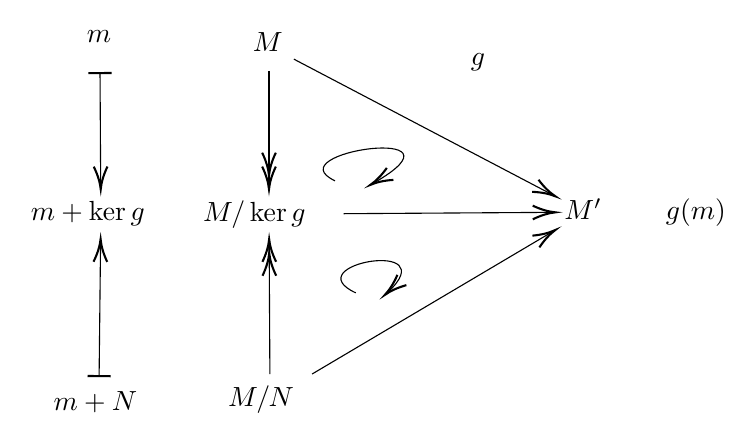
\begin{tikzpicture}[x=0.75pt,y=0.75pt,yscale=-1,xscale=1]
  %uncomment if require: \path (0,300); %set diagram left start at 0, and has height of 300

  %Curve Lines [id:da06639929221173313]
  \draw    (291.8,208.9) .. controls (262.25,195.11) and (335.54,182.29) .. (307.17,208.67) ;
  \draw [shift={(305.8,209.9)}, rotate = 318.81] [color={rgb, 255:red, 0; green, 0; blue, 0 }  ][line width=0.75]    (10.93,-3.29) .. controls (6.95,-1.4) and (3.31,-0.3) .. (0,0) .. controls (3.31,0.3) and (6.95,1.4) .. (10.93,3.29)   ;
  %Curve Lines [id:da2113069658179978]
  \draw    (281.8,154.9) .. controls (252.1,141.04) and (350.79,127.18) .. (300.37,156.01) ;
  \draw [shift={(298.8,156.9)}, rotate = 330.95] [color={rgb, 255:red, 0; green, 0; blue, 0 }  ][line width=0.75]    (10.93,-3.29) .. controls (6.95,-1.4) and (3.31,-0.3) .. (0,0) .. controls (3.31,0.3) and (6.95,1.4) .. (10.93,3.29)   ;

  % Text Node
  \draw (241,82.4) node [anchor=north west][inner sep=0.75pt]    {$M$};
  % Text Node
  \draw (391,162.4) node [anchor=north west][inner sep=0.75pt]    {$M'$};
  % Text Node
  \draw (346,92.4) node [anchor=north west][inner sep=0.75pt]    {$g$};
  % Text Node
  \draw (217,163.4) node [anchor=north west][inner sep=0.75pt]    {$M/\ker g$};
  % Text Node
  \draw (229,252.4) node [anchor=north west][inner sep=0.75pt]    {$M/N$};
  % Text Node
  \draw (145,255.4) node [anchor=north west][inner sep=0.75pt]    {$m+N$};
  % Text Node
  \draw (134,163.4) node [anchor=north west][inner sep=0.75pt]    {$m+\ker g$};
  % Text Node
  \draw (161,81.4) node [anchor=north west][inner sep=0.75pt]    {$m$};
  % Text Node
  \draw (440,162.4) node [anchor=north west][inner sep=0.75pt]    {$g( m)$};
  % Connection
  \draw    (262,96.3) -- (386.23,161.46) ;
  \draw [shift={(388,162.39)}, rotate = 207.68] [color={rgb, 255:red, 0; green, 0; blue, 0 }  ][line width=0.75]    (10.93,-3.29) .. controls (6.95,-1.4) and (3.31,-0.3) .. (0,0) .. controls (3.31,0.3) and (6.95,1.4) .. (10.93,3.29)   ;
  % Connection
  \draw    (250,102) -- (250,159) ;
  \draw [shift={(250,159)}, rotate = 270] [color={rgb, 255:red, 0; green, 0; blue, 0 }  ][line width=0.75]    (17.64,-3.29) .. controls (13.66,-1.4) and (10.02,-0.3) .. (6.71,0) .. controls (10.02,0.3) and (13.66,1.4) .. (17.64,3.29)(10.93,-3.29) .. controls (6.95,-1.4) and (3.31,-0.3) .. (0,0) .. controls (3.31,0.3) and (6.95,1.4) .. (10.93,3.29)   ;
  % Connection
  \draw    (250.43,248) -- (250.07,183) ;
  \draw [shift={(250.07,183)}, rotate = 449.68] [color={rgb, 255:red, 0; green, 0; blue, 0 }  ][line width=0.75]    (17.64,-3.29) .. controls (13.66,-1.4) and (10.02,-0.3) .. (6.71,0) .. controls (10.02,0.3) and (13.66,1.4) .. (17.64,3.29)(10.93,-3.29) .. controls (6.95,-1.4) and (3.31,-0.3) .. (0,0) .. controls (3.31,0.3) and (6.95,1.4) .. (10.93,3.29)   ;
  % Connection
  \draw    (270.77,248) -- (386.28,179.6) ;
  \draw [shift={(388,178.59)}, rotate = 509.37] [color={rgb, 255:red, 0; green, 0; blue, 0 }  ][line width=0.75]    (10.93,-3.29) .. controls (6.95,-1.4) and (3.31,-0.3) .. (0,0) .. controls (3.31,0.3) and (6.95,1.4) .. (10.93,3.29)   ;
  % Connection
  \draw    (286,170.76) -- (386,170.11) ;
  \draw [shift={(388,170.1)}, rotate = 539.62] [color={rgb, 255:red, 0; green, 0; blue, 0 }  ][line width=0.75]    (10.93,-3.29) .. controls (6.95,-1.4) and (3.31,-0.3) .. (0,0) .. controls (3.31,0.3) and (6.95,1.4) .. (10.93,3.29)   ;
  % Connection
  \draw    (168.15,249) -- (168.85,185) ;
  \draw [shift={(168.87,183)}, rotate = 450.62] [color={rgb, 255:red, 0; green, 0; blue, 0 }  ][line width=0.75]    (10.93,-3.29) .. controls (6.95,-1.4) and (3.31,-0.3) .. (0,0) .. controls (3.31,0.3) and (6.95,1.4) .. (10.93,3.29)   ;
  \draw [shift={(168.15,249)}, rotate = 450.62] [color={rgb, 255:red, 0; green, 0; blue, 0 }  ][line width=0.75]    (0,5.59) -- (0,-5.59)   ;
  % Connection
  \draw    (168.59,103) -- (168.91,157) ;
  \draw [shift={(168.93,159)}, rotate = 269.65] [color={rgb, 255:red, 0; green, 0; blue, 0 }  ][line width=0.75]    (10.93,-3.29) .. controls (6.95,-1.4) and (3.31,-0.3) .. (0,0) .. controls (3.31,0.3) and (6.95,1.4) .. (10.93,3.29)   ;
  \draw [shift={(168.59,103)}, rotate = 269.65] [color={rgb, 255:red, 0; green, 0; blue, 0 }  ][line width=0.75]    (0,5.59) -- (0,-5.59)   ;

  \end{tikzpicture}
\end{remark}
\begin{proposition} Dados dos $A$-módulos $M$ y $N$, existe un $A$-módulo $M\otimes_AN$ y una aplicación $A$-bilineal $\delta:M\times N\rightarrow M\otimes_AN$ tal que para cada $A$-módulo $P$ y para cada $F:M\times N\rightarrow P$ $A$-bilineal, existe una única aplicación $A$-lineal $f:M\otimes_AN:\rightarrow P$ tal que $f\circ\delta =F$.

Además, el par $(\delta,M\otimes_AN)$ es único, en el sentido que de existir otro par $(\delta',T)$ que verifique las condiciones del enunciado, se tiene que $T\cong M\otimes_AN$.

Al $A$-módulo $M\otimes_AN$ se le llama producto tensorial de $M$ y $N$.
\end{proposition}
\begin{proof}
Para ver la unicidad, supongamos que $(\delta,T)$ y $(\delta',T')$  cumplen las condiciones de la proposición. Poniendo a $T'$ como $P$ y a $\delta'$ como $F$, el resultado garantiza la existencia de $j:T\rightarrow T'$ tal que $\delta'=j\circ\delta$. Intercambiando los roles de $T$ y $T'$, se tiene $j':T'\rightarrow T$ tal que $\delta=j'\circ\delta'$. Entonces, cada una de las composiciones $j\circ j'$ y $j'\circ j$ son la identidad, lo cual garantiza que $j$ sea un isomorfismo.

Para la existencia, procedemos como sigue. Consideremos $A^{(M\times N)}$, la suma directa de $A$ tantas veces como elementos tenga $M\times N$. Definimos el siguiente subconjunto de $A^{(M\times N)}$ $$S=\{e_{(m+m',n)}-e_{(m,n)}-e_{(m',n)}, e_{(m,n+n')}-e_{(m,n)}-e_{(m,n')}, e_{(m,\lambda n)}-\lambda e_{(m,n)}, e_{(\lambda m,n)}-\lambda e_{(m,n)}\}$$   con $m,m'\in M$, $n,n'\in N$ y $\lambda\in A$.

Ahora tomamos $\Sigma$ el submódulo generado por $S$. Se cumple $\Sigma\subset A^{(M\times N)}$, luego podemos definir el cociente $A^{(M\times N)}/\Sigma$, que es un $A$-módulo. Entonces, definimos
$$\begin{array}{rcl}
    M\times N&\overset{\delta}{\longrightarrow}&\faktor{A^{(M\times N)}}{\Sigma}\\
    (m,n)&\longmapsto&[e_{(m,n)}]
    \end{array}$$
Ver que $\delta$ es bilineal es trivial por cómo se ha definido $S$. Por ejemplo, dados $m,m'\in M$, $n\in N$, $\delta(m+m',n)=[e_{(m+m',n)}]=[e_{(m,n)}+e_{(m',n)}]=[e_{(m,n)}]+[e_{(m',n)}]=\delta(m,n)+\delta(m',n)$.

Ponemos $M\otimes_AN=A^{(M\times N)}/\Sigma$. Definimos
$$\begin{array}{rrcl}
	f_0:&A^{M\times N}&\longrightarrow&P  \\
	&e_{(m,n)}&\longmapsto&F(m,n)
	\end{array}$$
que está bien definida ya que $\{e_{(m,n)}:(m,n)\in M\times N\}$ es un sistema de generadores de $A^{M\times N}$. Nótese que entonces $\{[e_{(m,n)}]: (m,n)\in M\times N\}$ es un sistema de generadores de $M\otimes_AN$. Por ser $F$ homomorfismo, $f_0$ es homomorfismo de $A$-módulos.

Veamos que $\Sigma\subset ker(f_0)$. Com $\Sigma$ está generado por $S$, basta ver $S\subset ker(f_0)$. Pero esto es directo por ser $F$ bilineal y la definición de $S$. Por ejemplo, $$f_0(e_{(m+m',n)}-e_{(m,n)}-e_{(m',n)})=F(e_{(m+m',n)}-e_{(m,n)}-e_{(m',n)}=0$$
Por tanto, siguiendo la observación anterior a la proposición, podemos definir
$$\begin{array}{rrcl}
	\tilde{f_0}:&\faktor{A^{M\times N}}{\Sigma}&\longrightarrow&P  \\
	&[e_{(m,n)}]&\longmapsto&F(m,n)
	\end{array}$$
que está bien definida y cumple las condiciones del teorema.
\end{proof}
\begin{remark}
\texit{1)} A las clases $[e_{(m,n)}]$ se les denota $m\otimes_An$ o simplemente $m\otimes n$.

Todo elemento de $M\otimes_AN$ es suma $\sum_{i=1}^rm_j\otimes n_j$, para ciertos $m_j\in M$, $n_j\in N$ y $r\in\mathbb{N}$, ya que $[\lambda e_{(m,n)}]=[e_{(\lambda m,n)}]=[e_{(m,\lambda n)}]$ por la definición inicial de $S$.

\textit{2)} Las aplicaciones bilineales de $M\times N$ en $P$, $Bil_A(M\times N,P)$ están en correspondencia biyectiva con $Hom_A(M\otimes_AN,P)$.

En particular, si tomamos $A$ como $K$ cuerpo y $M$ y $N$ $K$-espacios vectoriales,$$Hom_A(M\otimes_KN,K)=(M\otimes_KN)^{\ast}=Bil_K(M\times N,K)$$
\end{remark}
La construcción del producto tensorial de módulos se puede generalizar. Dados $M_1,\dots,M_r$ $A$-módulos, existe un $A$-módulo $M_1\otimes_A\dots\otimes_AM_r$ y$$\delta:M_1\times\dots\times,M_r\longrightarrow M_1\otimes_A\dots\otimes_AM_r$$ multilineal tal que para cualquier $$\Phi:M_1\times\dots\times,M_r\longrightarrow P$$ $A$-multilineal, existe una única $$f:M_1\otimes_A\dots\otimes_AM_r\longrightarrow P$$ $A$-lineal tal que $f\circ\delta=F$

En estas construcciones se tienen las siguientes propiedades.\begin{itemize}
    \item [1)] Dados $M_1,M_2$ y $M_3$ $A$-módulos, $M_1\otimes_AM_2\otimes M_3\overset{isom}{\cong}(M_1\otimes_AM_2)\otimes_AM_3\overset{isom}{\cong}M_1\otimes_A(M_2\otimes_AM_3)$
    \item [2)] $M\otimes_AN=N\otimes_AM$
    \item [3)] Dados $f:M_1'\rightarrow M_1$ y $g:M_2'\rightarrowM_2$ $A$-lineales, existe $f\otimes g:M_1'\otimes_AM_2'\rightarrow M_1\otimes M_2$ $A$-lineal tal que el diagrama es conmutativo.

    En particular, si $M\in Obj(Mod_A)$, $M\otimes\_$ es un funtor covariante de $Mod_A$ en $Mod_A$ (Véase Apéndice A)
    \end{itemize}
\end{document}
